%---------------------------------------------------------------------------------
%                西南交通大学研究生学位论文:第四章内容
%---------------------------------------------------------------------------------
\chapter{TCP/NC的改进及真实环境测试}
本章主要对文献\cite{Sundararajan2009}所提的TCP/NC给出几点改进,实现增强TCP/NC协议,即E-TCP/NC,并验证相关性能。提出了前向重传机制以应对一个RTO内的突发丢包;提出了一种新的自适应冗余度算法以应对网络的变化;对冗余包的发送时机给出改进以降低平均解码时延;设计补偿重传机制以降低解码端解码矩阵维度和减小解码时延。
\section{前向重传机制}
\subsection{TCP/NC的突发丢包问题}
通过冗余编码,TCP/NC可以很好地应对随机丢包网络的丢包。但当突发丢包发生时,TCP/NC表现就不好了。当突发丢包产生时,一般会要求重传,而TCP/NC的报文重传任务完全依赖TCP层。为了提高TCP/NC在突发丢包网络中的性能,本文提出了一种前向重传机制,能够同时高效地重传多个报文。
\par
通过增大TCP/NC的编码窗口可以提高TCP/NC应对突发丢包的能力,但是带来的后果是解码端运算复杂度的急剧增加,进而增大解码时延。在未发生超时重传时,TCP层单个、按序地在多个RTT内重传各个丢失的报文,因此TCP/NC会消耗很长一段时间来重传丢失的报文。图\ref{FR_EPS}展示了在丢了4个报文的情况下,TCP/NC是如何重传丢失的报文的。图\ref{FR_EPS}例子中设定的编码窗口值为2,冗余度为$\frac{1}{7}$,也就是说每7个编码包,多发一个冗余包。可以看到源端对$p_2$,$p_3$,$p_4$的重传总共耗费了3个RTT,导致目的端的NC层虽然在收到$C\left[8\right]$时就开始可以解码$p_5$后面的报文,但由于乱序,无法将它们上交给上层的TCP。
\par
在TCP-Reno中,对于重复ACK采取的是快速重传的方法。以图\ref{FR_EPS}为例,源端的NC层在收到3个对$p_2$的ACK之后,直接将其交付给上层TCP。上层TCP收到3个重复的对$p_2$的ACK,认为报文$p_2$丢失了,采取快速重传,只重传$p_2$,然后进入拥塞避免阶段,继续接着$p_{10}$发送$p_{11}$。接收端在收到$p_2$的重传报文$C\left[11\right]$后,又陆续回给源端多个重复ACK,表示$p_3$丢失。源端TCP又启动快速重传,重传报文$p_3$。后面对报文$p_4$的重传和$p_1$,$p_2$的情况一样。当编码窗口的值更大,RTT比较大时,这种情况产生的影响更大。
\par
TCP-Reno对于一个RTO内报文的连续丢失采取的是单个依次重传的处理策略,因此对突发丢包不是很友好。NC层的引入让这一策略的劣势更为凸显。当NC层出现重复ACK时,意味着链路中出现的丢包就绝不仅仅是单个报文的丢失,这是由于NC层的“seen”机制导致的。直觉上,由于NC层缓存有未被确认的数据包,我们可以在NC层重传那些未被看到的报文。当NC层收到第一个从TCP层下来的重传报文\emph{pkt}后,NC层不仅重传\emph{pkt},而是会在一个RTT内顺便将所有未看到的报文都重传。如此,可以让上层TCP认为仅仅就丢了一个包。如图\ref{NEWFR_EPS}所示,NC层收到上层TCP的重传报文$p_2$后,在一个RTT内重传了未看到的报文$p_2$,$p_3$和$p_4$。
\begin{figure}[htbp]
	\centering
	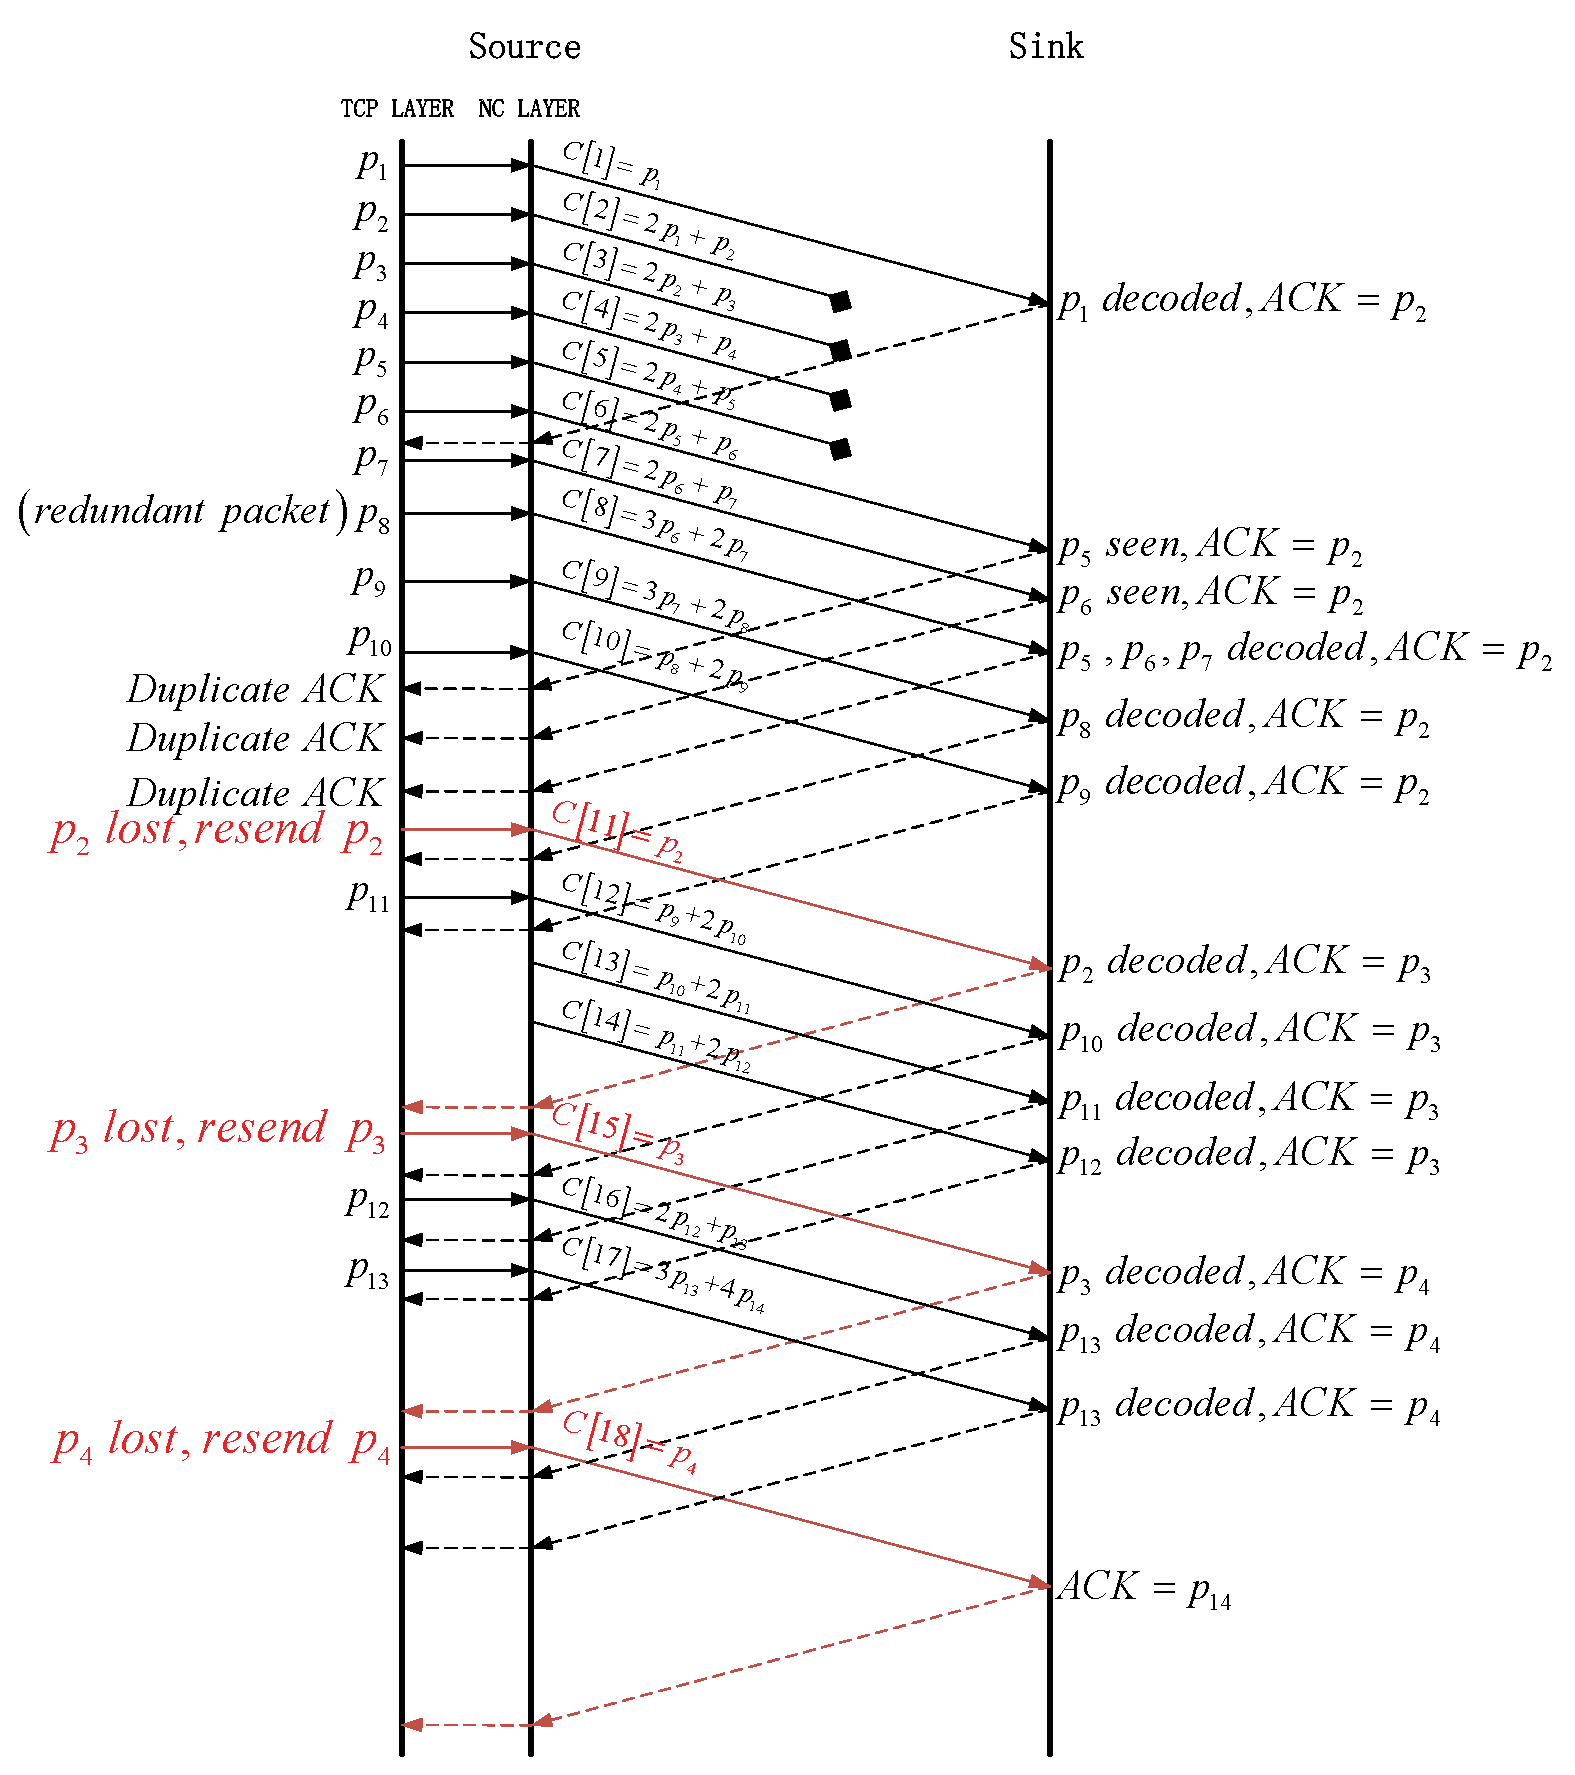
\includegraphics[width=4in]{figures/fr.eps}
	\caption{原有TCP/NC的重传机制}
	\label{FR_EPS}
\end{figure}
\begin{figure}
	\centering
	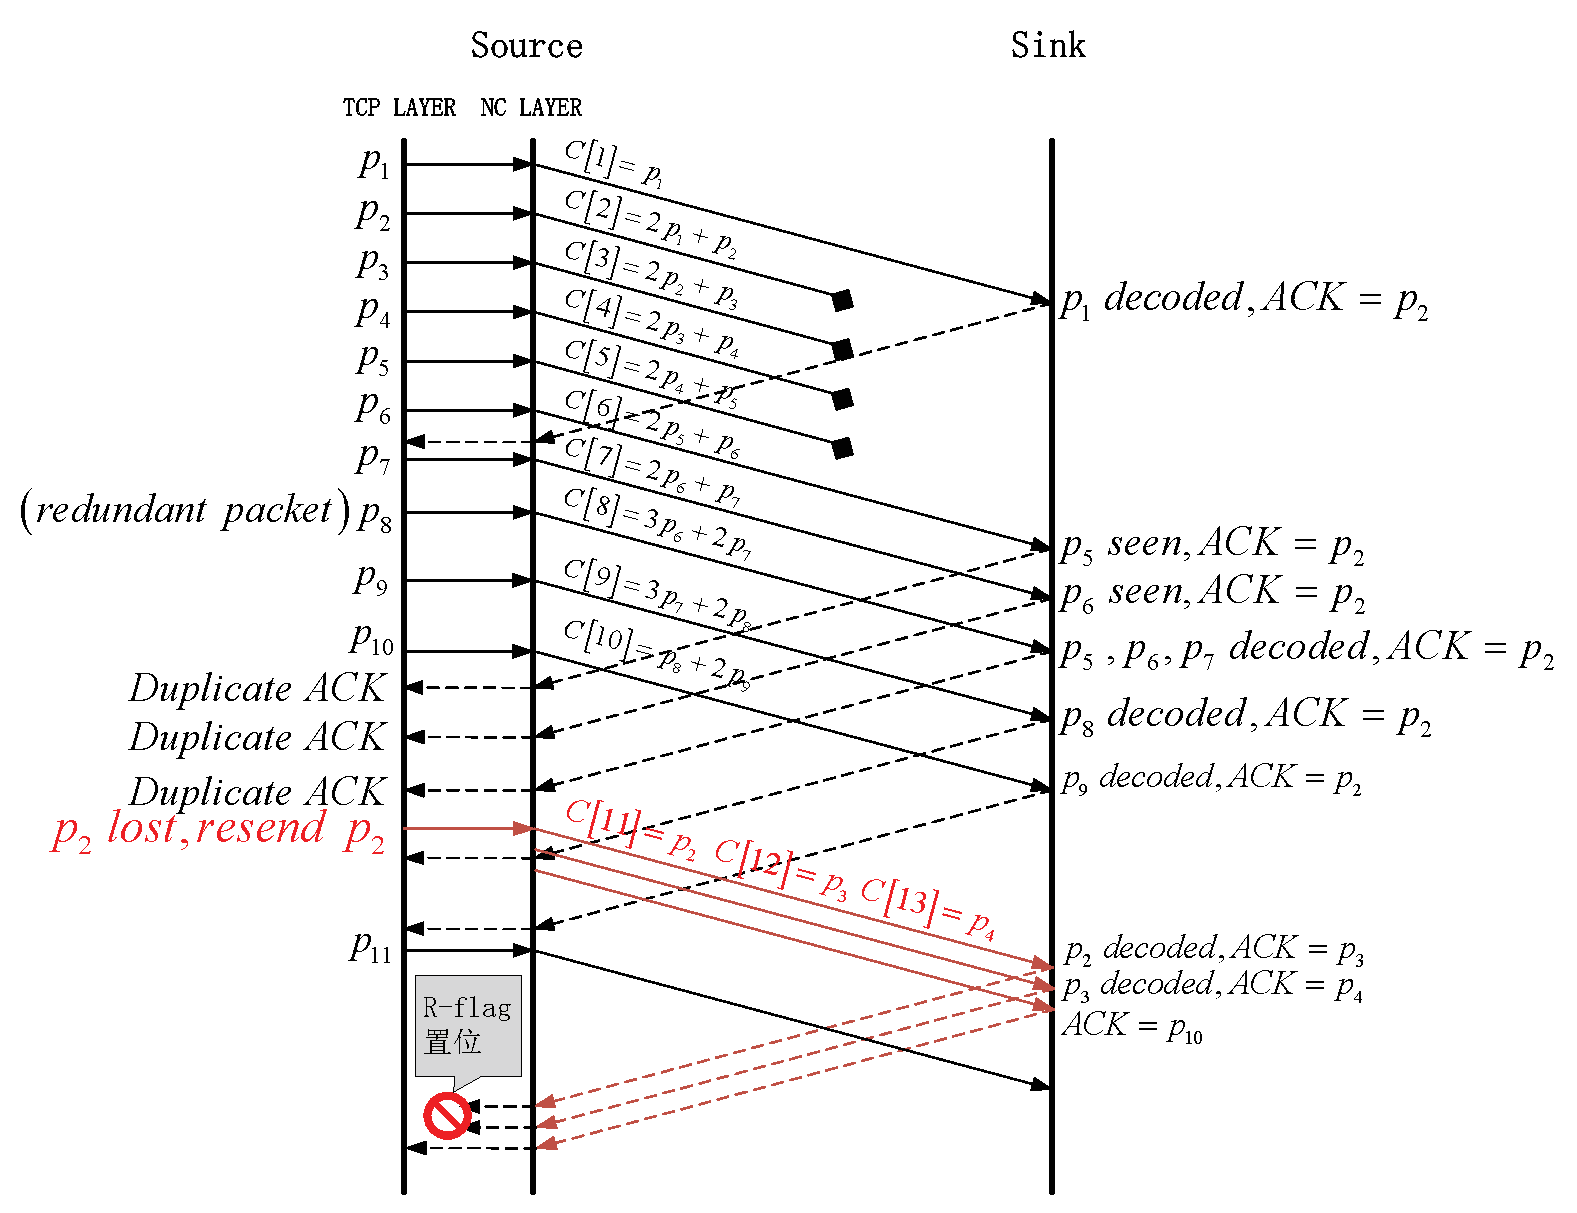
\includegraphics[width=4in]{figures/newfr.eps}
	\caption{前向重传机制}
	\label{NEWFR_EPS}
\end{figure}
\subsection{新NC头部设计}
为了支撑前向重传机制,本文设计了新的NC头部,如图\ref{NEWHEADER_EPS}。原有TCP/NC头部设计 ( 图\ref{CODINGHEADER_EPS} )中的Res字段,有6个比特可供使用,对应图\ref{NEWHEADER_EPS}中的$b_1 \sim b_6$。此六个比特与标准TCP中的保留字段对应。在第\ref{ztlc}小节中,我们讲到需要区分NC报文和普通TCP报文,可以利用$b_1$标识这个是TCP报文还是NC报文。利用$b_2$表示R-flag,表示当前这个报文是否要被上交给TCP层;利用$b_3$、$b_4$和$b_5$一起表示当前报文的\emph{报文状态}( 后面会讲到\emph{报文状态}的作用 )。增加了Pid和Pid-reply两个域,各自两个字节。其中Pid表示NC层发出的报文编号,以报文为计数单位,而非字节。NC层发出的每个线性组合报文有独一无二的Pid( 回环问题另做考虑 ),接收端在收到编号为Pid的线性组合报文后,在回复的ACK报文中,Pid-reply域就填上Pid,表示当前这个ACK是由编号为Pid的线性组合包激发的。
\begin{figure}[htbp]
	\centering
	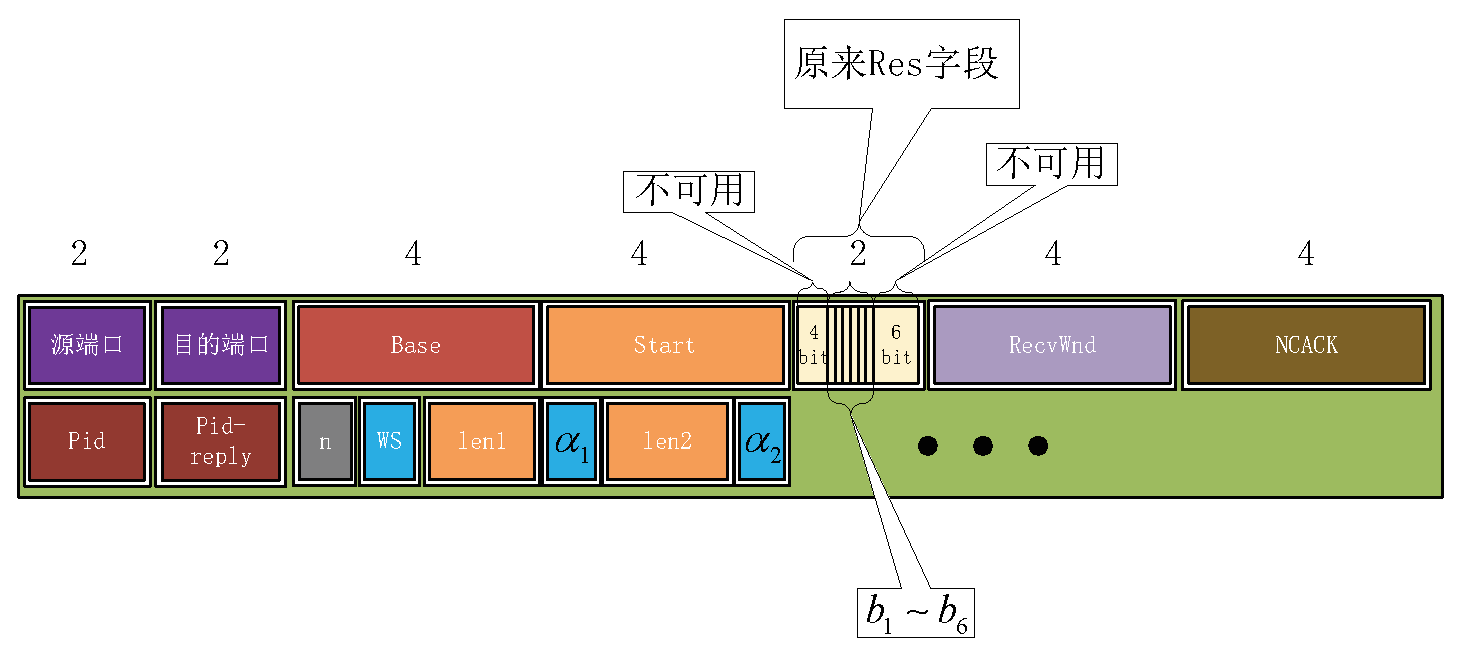
\includegraphics[width=6in]{figures/newheader.eps}
	\caption{新NC头部设计}
	\label{NEWHEADER_EPS}
\end{figure}
\subsection{定位丢包}\label{DWDB}
为了在NC层重传未被看到的报文,首先需要确定丢了哪些报文。
\par
源端保存了每个编码包的原始数据包信息,即这个编码包是由哪几个原始数据包组成的,如图\ref{FR_EPS}中的$C\left[9\right]$由$p_7$和$p_8$组成。当发送端收到接收端回复的ACK报文时,有如下几种情形。
\begin{enumerate}[fullwidth,itemindent=2em,label=(\arabic*)]
	\item 有新的数据被确认且ACK报文中R-flag( 后面会解释R-flag含义 )未置位,那么将其交给上层TCP。
	\item 有新的数据被确认而ACK报文中R-flag置位,此ACK需要被抑制,不会被交付给上层TCP,如图\ref{NEWFR_EPS}中对$C\left[11\right]$和$C\left[12\right]$的ACK,但会更新NC层中未被看到的报文,从未被看到的报文列表中移除本次新确认的数据。
	\item 本次ACK并没有确认新的数据,提取其中的\emph{Pid-reply}域,然后罗列Pid值为Pid-reply的编码包的所有原始数据包$p_i \sim p_j(i \le j)$。如果目前在发送端未被确认的数据包中最小序号为$seq_1$,$p_i$数据包的起始序号是$seq_2$,那么我们可知接收端那边未看到的报文序号是在$seq_1 \sim \left(seq_2 - 1\right)$之间。由于发送端可能会收到接收端多个这样的ACK报文,如图\ref{NEWFR_EPS}中对$C\left[6\right]$,$C\left[7\right]$和$C\left[8\right]$的确认ACK报文,未看到的报文区间会被更新,但更新的方式只能是区间长度变小,也就是说$seq_2-1$只能向着$seq_1$靠拢。以图\ref{NEWFR_EPS}为例,发送端在收到对$C\left[7\right]$的ACK后,未看到的报文区间不会改变,依然是$seq_{p_2} \sim seq_{p_5} - 1$。
\end{enumerate}
\par
从图\ref{NEWFR_EPS}中可以看到,接收端发出的对报文$C\left[11\right]$和$C\left[12\right]$的确认ACK报文被发送端的NC层抑制了,并没有交给上层。发送端的NC层直到收到ACK为$p_{10}$的报文,才将此ACK上交给上层TCP。这样达到了让上层TCP以为仅仅丢了一个包的目的。因此,我们需要在NC头部添加\emph{报文状态}字段。可以告知接收端当前这个报文能否让接收端产生确认所有重传报文的ACK报文。如果可以,那么接收端在回复给发送端的ACK报文中会将R-flag清掉;如果不行,接收端在回复给发送端的ACK报文中会对R-flag置位。这样发送端的NC层就可以根据R-flag状态来决定是否将ACK报文送往上层TCP。表\ref{tab:BWZT}展示的是所有的报文状态信息。

\begin{table}[htp]
	\centering
	\caption{报文状态描述}
	\label{tab:BWZT}
	\begin{tabular}{l|l}
		\toprule
		报文状态( $b_3b_4b_5$) &描述\tabularnewline
		\midrule
		000		& 正常的编码包\tabularnewline
		001		& 冗余编码包 \tabularnewline
		010		& 未编码重传报文,但不是最后一个\tabularnewline
		011 	& 未编码重传报文,且是最后一个\tabularnewline
		100		& 重传编码报文,但不是最后一个\tabularnewline
		101		& 重传编码报文,且是最后一个\tabularnewline
		\bottomrule
	\end{tabular}
\end{table}
\subsection{重传丢包}
每当NC层收到上层TCP下来的重传报文时,我们的前向重传机制才会启动。发送端的NC层维护了一个链表\emph{re\_list},保存着接收端那边未看到的报文;\emph{re\_list}通过接收端那边回的ACK报文来更新。是否启动前向重传取决于\emph{re\_list}是否为空。当NC层完成前向重传后,\emph{re\_list}会被清空。
\par
值得注意的是,在重传过程中,对于\emph{re\_list}中的报文,我们发送的是原始数据包,例如图\ref{NEWFR_EPS}中的$p_2$、$p_3$和$p_4$。这是为了加快接收端的解码进程。对照表\ref{tab:BWZT},图\ref{NEWFR_EPS}中报文$p_2$和$p_3$的\emph{报文状态}域上填写的都是010;报文$p_4$的\emph{报文状态}域上填写的是011。这是由于$p_4$是这个非编码重传序列的最后一个重传报文。接收端在收到重传的$p_2$、$p_3$和$p_4$后会产生3个ACK报文,通过检查$p_2$、$p_3$和$p_4$的\emph{报文状态}域,接收端知道$p_4$才是这个非编码重传序列的最后一个重传报文。因此,对于$p_2$、$p_3$的ACK报文,接收端会对其R-flag域置位,让发送端的NC层不将$p_2$和$p_3$的ACK报文上传给TCP层;而对于$p_4$的ACK报文,接收端会清掉R-flag域,让发送端的NC层将$p_4$的ACK报文上传给TCP层。
\par
考虑一下重传报文丢失的情况。
\begin{enumerate}[fullwidth,itemindent=2em,label=(\arabic*)]
	\item 如果重传序列的第一个报文或者中间报文丢失,那么依然会触发重复ACK,情形退回到前向重传机制开始之前的情况。
	\item 如果最后一个重传报文,如$p_4$丢失,那么发送端只会收到R-flag置位的ACK报文,如$p_2$和$p_3$的ACK报文;由于R-flag置位,发送端的NC层不会将这些ACK报文上交给TCP层,但是会更新NC层的编码缓存;一段时间后上层TCP会重传刚刚才重传过的报文序列,如$p_2$、$p_3$和$p_4$;NC层发现$p_2$和$p_3$被接收端确认了,会立马创建一个ACK报文,回给上层TCP;NC层发现\emph{re\_list}为空,$p_4$不在\emph{re\_list}中,而$p_4$在编码缓存中,因此会将$p_4$加入到\emph{re\_list},重传$p_4$,并清空\emph{re\_list}。
\end{enumerate}
\par
考虑一下超时重传的情况。NC层通过检查TCP层下来的报文是否在编码缓存中来确定这个报文是否是重传包。不管是超时重传报文还是快速重传报文,都首先检查该报文是否在\emph{re\_list}中,如果不在就加入到\emph{re\_list},然后重传\emph{re\_list}的所有报文。
\subsection{编码重传包}
考虑到重传序列的最后一个重传包丢失造成的性能损失比较大,本文对重传报文进行再编码。在重传了\emph{re\_list}的所有不编码原始报文后,再重传$\left\lceil {R \times num\_re} \right\rceil  - num\_re$个编码报文,其中\emph{R}表示冗余度,\emph{num\_re}表示\emph{re\_list}中重传报文的个数。重传编码报文的\emph{报文状态}域填写方式参照表\ref{tab:BWZT}。
\section{改进冗余包发送时机}
文献\cite{Sundararajan2009}中冗余包分布并非均匀分布。给定一个固定冗余度,其冗余特性并没有体现在每个编码包中。因此本文重新设计了冗余包的发送时机。假定冗余度为\emph{R} ( $R \ge 1$ ),对于从TCP层下来的每个报文,以$R - \left\lfloor R \right\rfloor$的概率发送 $\left\lfloor R+1 \right\rfloor$个编码包;以$1-\left(R-\left\lfloor R \right\rfloor\right)$的概率发送$\left\lfloor R \right\rfloor$个编码包。这样冗余度均匀分布在每个数据包中了。
\section{自适应冗余度算法}
文献\cite{Sundararajan2009}中并没有给出冗余因子\emph{R}的设置规则。自觉告诉我们,将\emph{R}设置为一个常量值是不合适的。现实中的网络环境,尤其是无线环境,其丢包率是在变动的。在设置冗余因子时,如果\emph{R}过小,那么冗余信息不足以掩盖链路中的丢包;如果\emph{R}值过大,编码码率就过小,降低网络的有效吞吐率。因此需要找出一种能够根据网络状况自适应调整冗余度的方法,最大化地利用网络带宽。
\par
文献\cite{6261883}针对TCP/NC提出了一种自适应冗余算法。作者借鉴TCP-Vegas中的\emph{Vegas loss predictor}\textsuperscript{\cite{martignon2004loss,brakmo1995tcp}},在NC层实现了一个\emph{loss differentiation scheme}。通过估计当前的网络拥塞状态和收到的重复ACK信息,在让网络不出现拥塞的前提下可以动态调整冗余度。其缺点则是\emph{Vegas loss predictor}在面对TCP-Reno竞争时的无力\textsuperscript{\cite{hasegawa2000fairness}}。
\par
文献\cite{song2011self}设计了SANC-TCP,其基本思想是对产生的编码报文进行编号,在ACK的头部添加两个域\emph{loss}和\emph{echo\_pktID}。发送端根据接收到的ACK报文中的\emph{loss}和\emph{echo\_pktID},以及编码窗口的值来动态调整冗余度。其中\emph{loss}表示接收端的解码矩阵中序号最大的原始数据包编号和“seen packets”编号之间的差值;\emph{echo\_pktID}表示哪个报文激发了本次ACK。其在调整冗余度时不仅考虑了当前网络的丢包率,还将接收端的解码矩阵的状态信息考虑进去。
\par
考虑到在设计前向重传机制中引入的Pid和Pid-reply字段,本文依据Pid和Pid-reply设计了一个新的自适应冗余算法。由文献\cite{Sundararajan2011}中可知,冗余度\emph{R}与丢包率密$\rho$密切相关,理想情况下其关系为
\begin{equation}
	R=\dfrac{1}{1-\rho}
\end{equation}
因此需要知道当前链路的丢包率。可以由Pid和Pid-reply字段计算得到。如图\ref{DIUBAO_EPS}中展示,发送端提取接收到的ACK中的Pid-reply字段即可了解Pid=103的报文丢失了,进而计算在Pid=100到Pid=104时段内的丢包率$\rho=25\%$。需要注意如下几点:
\begin{figure}[htbp]
	\centering
	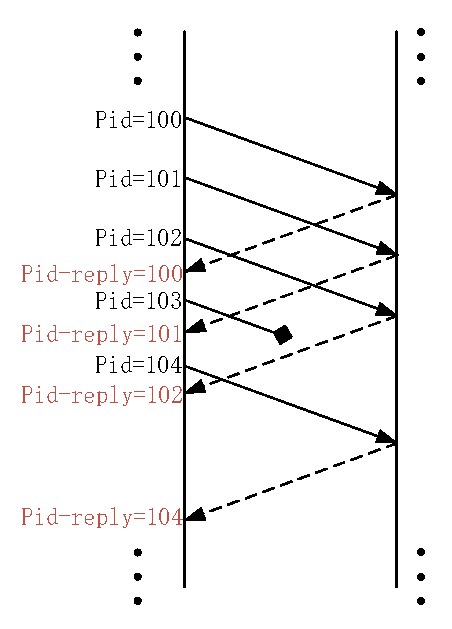
\includegraphics[width=2in]{figures/diubao.eps}
	\caption{计算丢包率示例}
	\label{DIUBAO_EPS}
\end{figure}
\begin{itemize}[leftmargin=.5in]
	\item 对于收到的每个编码包,接收端都会回复ACK,这会浪费一些带宽;
	\item 考虑到ACK报文丢失问题,我们计算得到的丢包率可能比实际情况大一些,但这影响不大;
	\item 接收端对于冗余包也需要回复ACK,并对其NC头部的R-flag置位,通知发送端的NC层不要将此ACK上传给TCP层
\end{itemize}
同时如第\ref{DWDB}小节所述,我们可以通过Pid-reply和ACK确认号来获知接收端的解码矩阵信息。换句话说,可以大概了解接收端的解码矩阵还差多少个编码包才可以变为可解状态。

\section{补偿重传算法}
\section{真实网络环境测试}
\subsection{无人机lossy信道环境搭建}
\subsection{测试结果}
\subsection{性能分析}
\section{本章小结}
为了在真实丢包环境中测试TCP/NC及其改进协议的性能,本文搭建了无人机测试环境。将部署了TCP/NC改进协议的Raspberry Pi搭载在无人机上,通过WIFI无线链路来与地面站通信。 